\subsection{Load Balancing}
Load Balancing ist eine wichtige Strategie, um die Leistung und Resilienz verteilter Systeme erheblich zu steigern. Hierfür wird die anstehende Arbeitslast dynamisch auf verfügbare Server oder Ressourcen aufgeteilt.

\subsubsection{Übersicht}
Drei Komponenten spielen hier eine wichtige Rolle. Im Mittelpunkt dieses Verfahrens steht der Load Balancer, eine Software- oder Hardwarekomponente, welche serverseitig über mehrere Dienste verwaltet. Die zweite Komponente ist eine Gruppe von gleichartigen Service-Instanzen, welche die eigentliche Geschäftslogik beinhalten. Eingehende Anfragen werden zuerst den Load Balancer gestellt, welcher diese dann mithilfe einer geeigneten Strategie möglichst gerecht auf die Service-Instanzen aufteilt.

Zuletzt ist eine Komponente von Nöten, welche verfolgt, wie viele Service-Instanzen in der Konstellation vorhanden sind und in welchem Zustand sich diese befinden, also Service Discovery bewerkstelligt. Dies erfolgt hier Server-Side: Ein Client hat keine Kenntnis über den Aufbau, also Topologie, dieses Systems \cite{schoner2017analyse}. Ob Load Balancing überhaupt Anwendung findet oder wie viele Ressourcen zur Verfügung stehen, wird nicht kommuniziert. Stattdessen geschieht jede externe Kommunikation nur mit dem Lastverteiler, welcher intern mithilfe der Registry ermittelt, welche Dienstknoten geeignet und bereit sind, die Anfrage entgegenzunehmen. Der Lastverteiler vermittelt nach Auswahl des Knotens schließlich zwischen dem Client und dem gewählten Service.

Load Balancing ist ebenso mit clientseitiger Service Discovery möglich. Hier existiert also kein zentraler Load Balancer, stattdessen ist der Client \textit{Registry-aware} \cite{schoner2017analyse} und wählt selbstständig einen passenden Serviceknoten aus, er verhält sich also selbst wie ein Load Balancer. Da die eigentliche Lastverteilungsmethodik dennoch ähnlich zur serverseitigen Discovery erfolgt und diese Methode speziell angepasste Clientsoftware benötigt, wird sie im weiteren Verlauf nicht näher erläutert.

\begin{figure}[t]
  \centering
  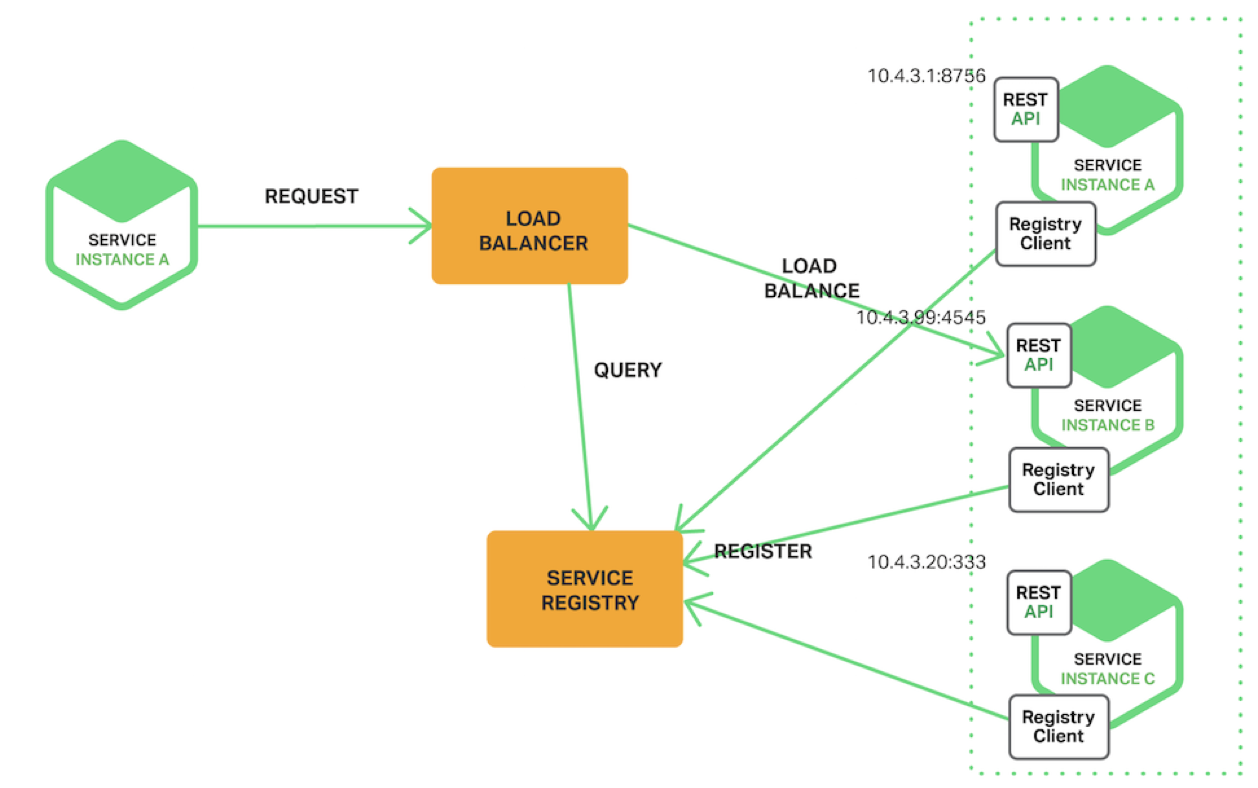
\includegraphics[width=\linewidth]{images/loadbalancer.png}
  \caption{Load Balancer mit drei Serviceinstanzen \cite{schoner2017analyse}}
    \label{fig:loadbalancer}
  \Description{Load Balancer mit Serverseitiger Service Discovery und drei Serviceinstanzen}
\end{figure}

In Abb.~\ref{fig:loadbalancer} werden die drei Komponenten mit dem typischen Datenfluss schematisch dargestellt: die Dienstinstanzen registrieren sich bei ihrem Start in der Service Registry. Erfolgt nun eine externe Anfrage an den Load Balancer, fragt dieser wiederum die Registry an, welche Dienste angemeldet sind. Mit dieser Information kann ein Dienst ausgewählt werden, und die eigentliche Anfrageverarbeitung kann stattfinden. Die Anfrage (Abb.~\ref{fig:loadbalancer}, links) erfolgt nie direkt an eine der Dienstinstanzen.
\subsubsection{Zustandsverfolgung der Dienste}
Im vorherigen Beispiel verfolgt die Service Registry zuerst nur, ob ein Service gestartet wurde. Dafür registriert bzw. deregistriert sich der Service zum Start oder planmäßigen Ende seiner Ausführung.

Um eine effektive Lastverteilung zu ermöglichen reicht diese Information jedoch nicht aus. Wenn das Balancing ausschließlich realisiert wird, indem alle Anfragen \glq blind\grq{} auf Serviceknoten verteilt werden, könnten zwei Szenarien eintreten:
\begin{itemize}
	\item Obwohl die gleiche Anzahl an Anfragen fair an mehrere Knoten verteilt wird, könnte ein Knoten überlastet werden. Möglich wäre dies, wenn die entsprechenden Anfragen zufällig rechenintensiver sind als die Anfragen an andere Knoten. Ebenso denkbar ist, dass auf der Serverhardware andere Dienste oder (im Fall eines virtualisierten Computers) parallel ausgeführte virtuelle Maschinen mehr Rechenzeit verbrauchen (sogenannte \glqq Noisy Neighbours\grqq{}). Analog könnte eine langsamere Netzwerkanbindung zu unterschiedlichen Kapazitäten zwischen Knoten führen.
	\item Ein Serviceknoten könnte versagen. Beispielsweise könnte er ansprechbar sein, aber nur noch Fehlermeldungen zurückgeben. Alternativ antwortet er womöglich gar nicht mehr, oder benötigt derart viel Zeit, dass die Anfragen zum Zeitpunkt der Fertigstellung nicht mehr von Nutzen sind.
\end{itemize}

Es ist ersichtlich, dass ein pures Aufteilen der Anfragen auf die Serviceknoten ohne Einsicht in deren Zustände nicht sinnvoll ist. Aus diesem Grund wird die Service Registry erweitert um sogenannte \textit{Health Checks}: Jede Serviceinstanz kommuniziert ihre Auslastung und etwaige Fehler, und der Lastverteiler kann daraufhin sinnvolle Entscheidungen treffen.
%In beiden Fällen würde die Lastverteilung 

\subsubsection{Strategien der Lastverteilung}
Die Auswahl eines Serviceknoten bei der Lastverteilung kann prinzipiell auf zwei Wege erfolgen. Bei der statischen Lastverteilung wird die aktuelle, tatsächliche Auslastung eines Knoten nicht beachtet, die Last wird stattdessen \glq blind\grq\ verteilt, und lediglich das Bereitsein der Knoten wird berücksichtigt \cite{mishra.2020}. Beispiele statischer Strategien sind Round Robin, bei welcher anstehende Aufgaben zyklisch auf die Instanzen verteilt werden, oder das Load Balancing mit Hashing der Anfragen-IP-Adresse, bei welcher die Serviceknoten praktisch zufällig gewählt werden während mehrere Anfragen der gleichen Quelle immer auf dem gleichen Serviceknoten verarbeitet werden \cite{g4g-loadbalancing}.
\todo{im vergleich redundanz/partit./skal. bewerten}

Die dynamische Lastverteilung hingegen berücksichtigt die Momentanauslastung eines Serviceknotens. Gängige Strategien sind
\begin{itemize}
	\item Least Connection Load Balancing: Eine anstehende Aufgabe wird dem Dienst übergeben, welcher momentan die wenigsten aktiven Netzwerkverbindungen hat.
	\item Least Response Time Load Balancing: Die benötigte Zeit zur Vollendung der letzten Anfragen wird pro Serviceknoten protokolliert. Der Knoten, der historisch am schnellsten ist, erhält die nächste Aufgabe.
	\item Resource Based Load Balancing: Alle Serviceknoten berichten ihre aktuelle Auslastung anhand generischer Merkmale wie die CPU- oder Arbeitsspeicherauslastung. Dem Knoten mit der niedrigsten Auslastung wird die nächste Aufgabe zugewiesen.
\end{itemize}















